\chapter{Vehicle Model Exercises}

\section{Exercise 1 - Vehicle Model Implementation}

\textbf{Q. For each maneuver, plot and comment the main results that you obtain, particularly focusing on tire forces and moments (\{$\fx$, $\fy$, $\fz$, $\mz$\}) and tire slips (\{$\kappa$, $\alpha$\}).}

\begin{enumerate}
  \item initial conditions: $\uz$ = 30 km/h \\
simulation timing: $\ts$\ = 0.001 s, $\tf$\ = 20 s \\
requested pedal: req\_pedal = 1 \\
requested steering wheel angle: req\_steer = 0 deg.
  \end{enumerate}
  
        \begin{figure}[ht]
        
\includegraphics[width=0.99\linewidth]{ex4/q1/ex-41b.eps}
        \centering
        \caption{vehicle motion graphs [maneuver \#1]}
        \label{41b}
        \end{figure}

Figure \ref{41b} shows the motion graphs of the first maneuver. The vehicle starts from 30 km/h, with no steering input and full throttle. The velocity increased until it reached full speed of 108 km/h within 5 seconds. All upcoming graphs are influenced by the acceleration profile.

        \begin{figure}[ht]
        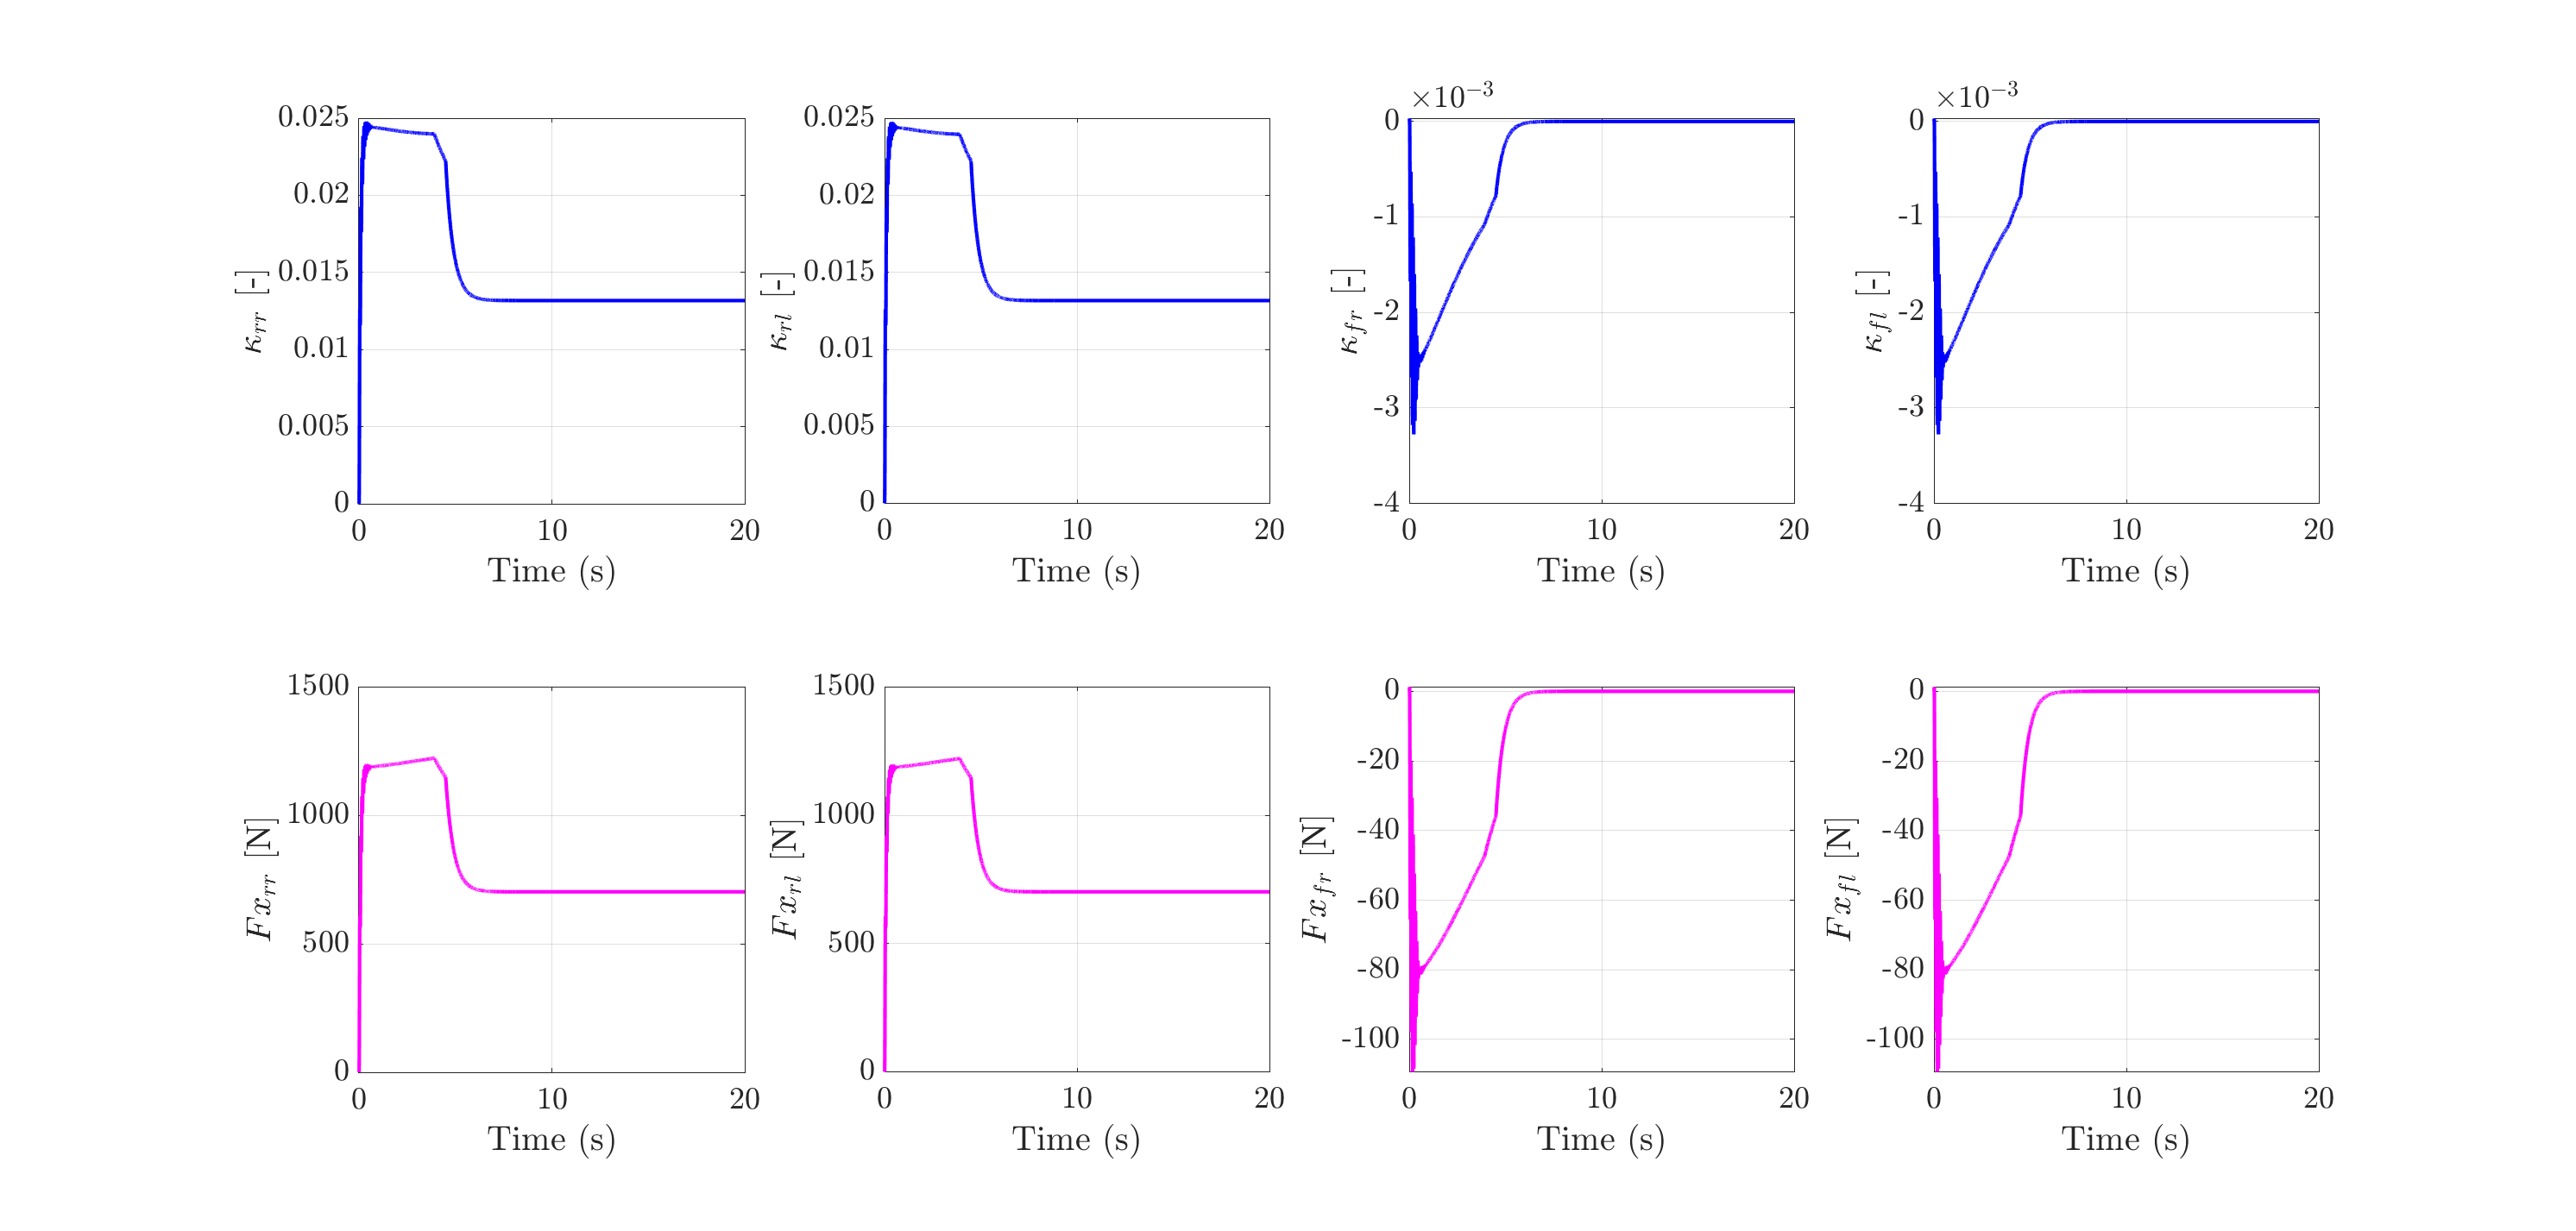
\includegraphics[width=0.85\linewidth]{ex4/q1/ex-41f.eps}
        \centering
        \caption{longitudinal slip $\kappa$ and longitudinal forces $\fx$ [maneuver \#1]}
        \label{41f}
        \end{figure}
        
The graphs in Figure \ref{41f} shows no difference between both right tires [and similarly the left tires] as the vehicle was moving straight without steering input. However, both rear tires show much higher $\kappa$ and $\fy$. This was expected as the vehicle is rear-wheel drive and torque applied from the motors would increase both the slip and force experienced by the rear tires.

During the vehicle's acceleration to maximum speed [between 0 and 5 seconds] all tires showed higher slip and force. Once maximum speed is reached [acceleration is zero], the slips and forces decrease across all tires. The front tires go to zero, while the rears do not, as the motors must still keep applying [decreased] torque to keep the vehicle at speed.

        \begin{figure}[ht]
        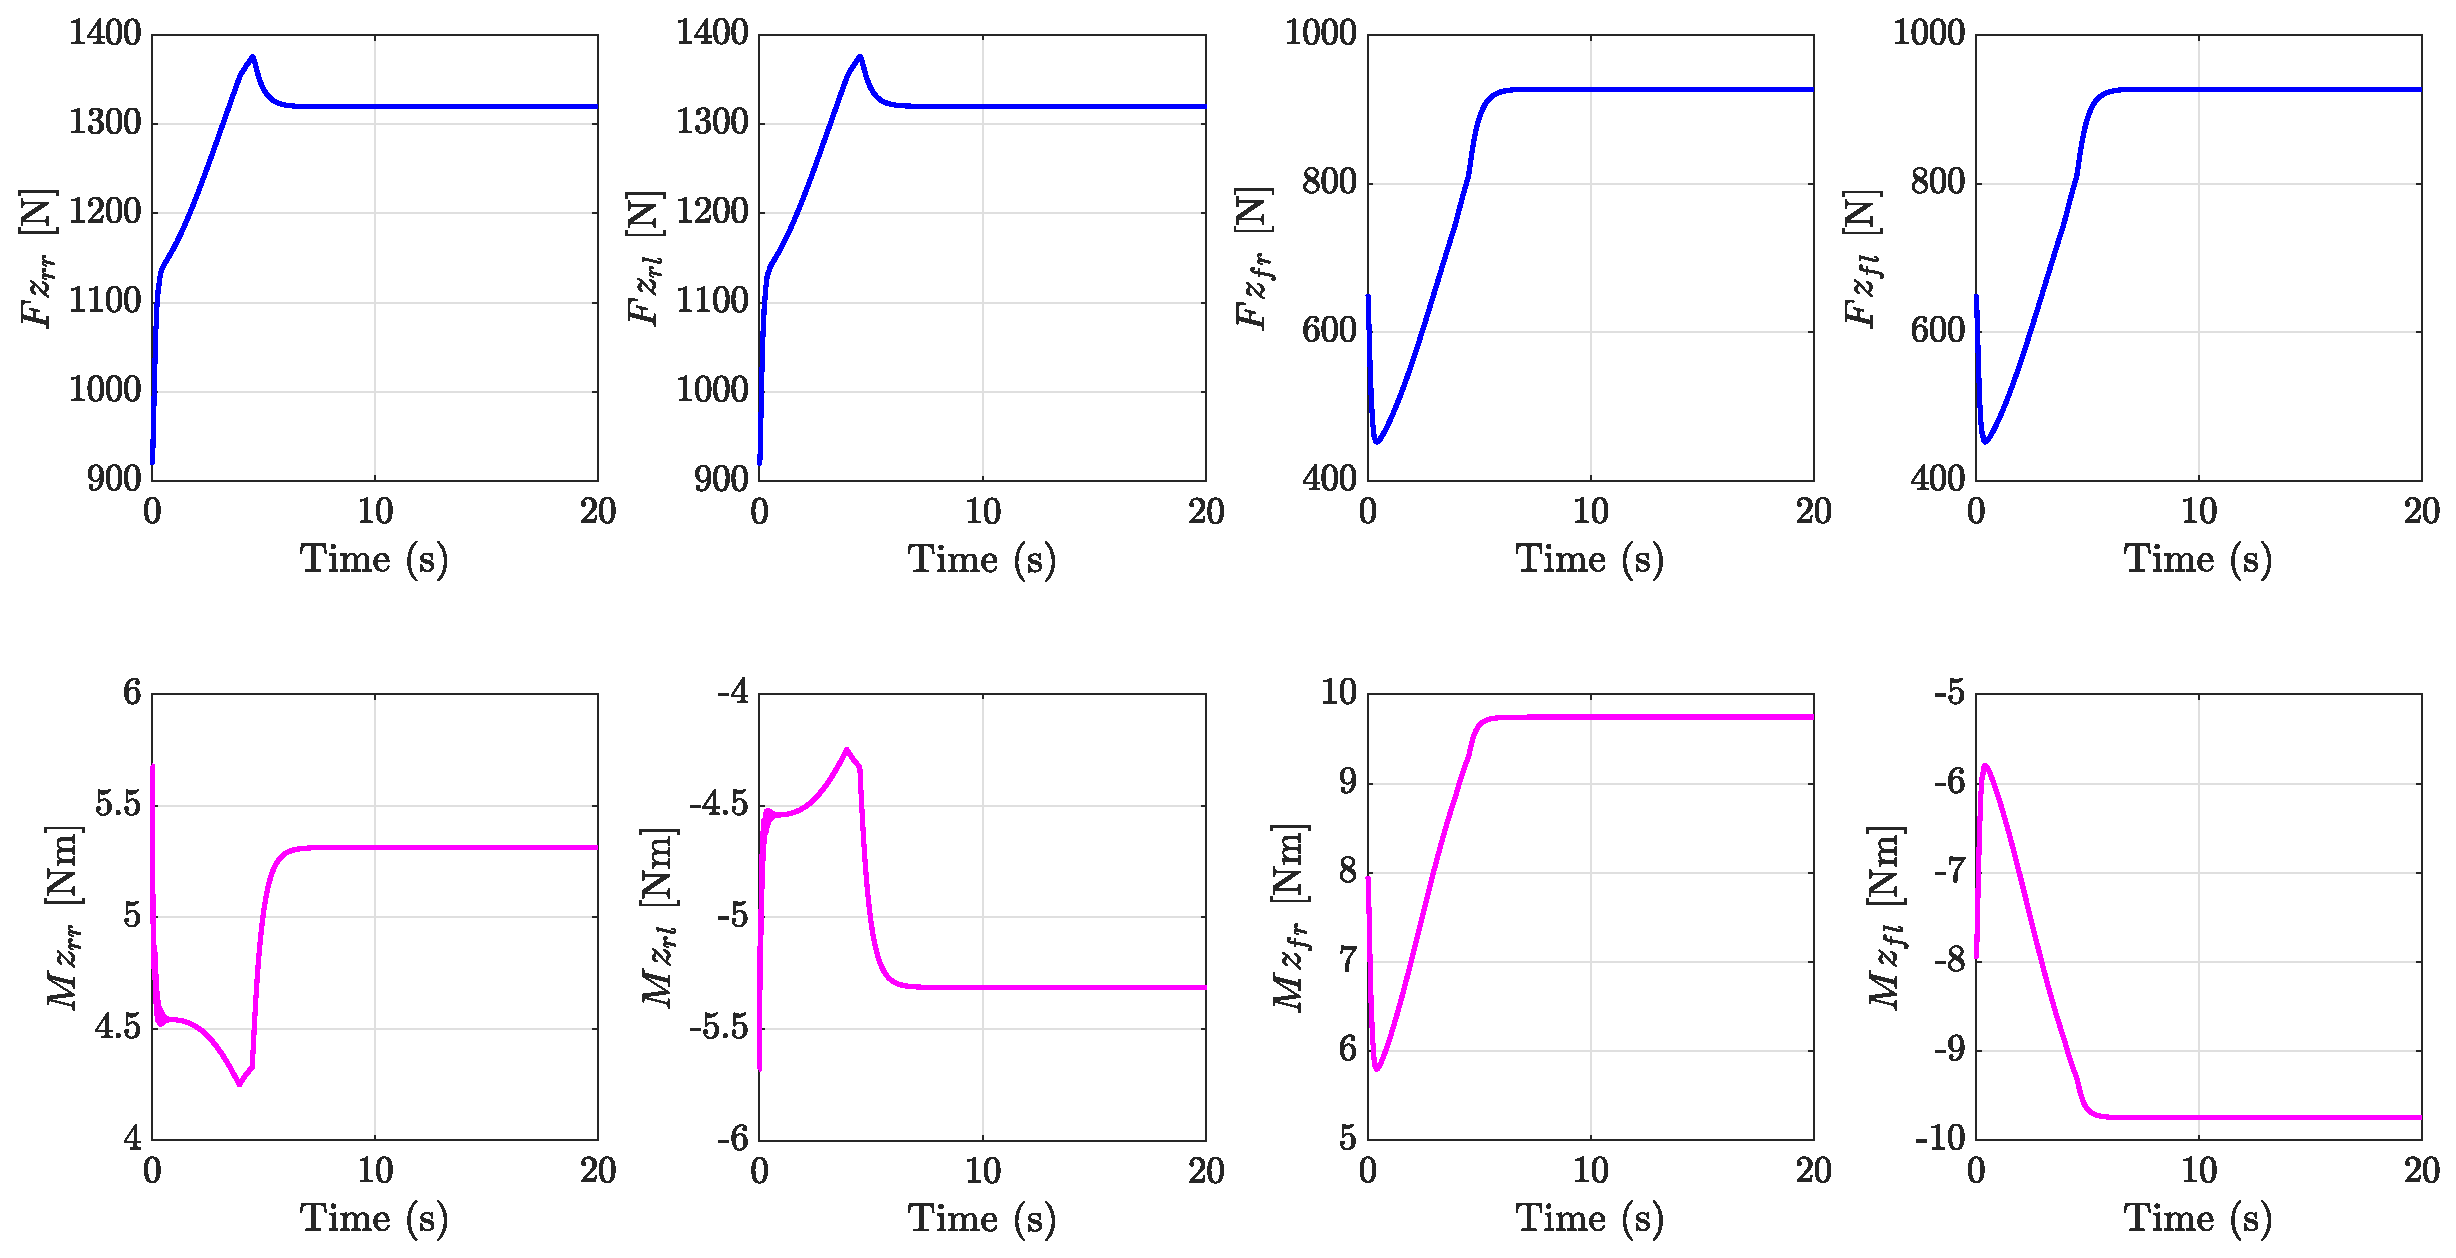
\includegraphics[width=0.85\linewidth]{ex4/q1/ex-41h.eps}
        \centering
        \caption{Vertical forces $\fz$\ and self aligning torque $M_{z}$ [maneuver \#1]}
        \label{41h}
        \end{figure}
        
The aerodynamics load $\fa$\ increases as speed increases. As shown in Figure \ref{41h}, the vertical force $\fz$ increases across all tires because it relies on $\fa$. The vertical loads are calculated using Equation \ref{eq:4.1}:

\begin{equation}\label{eq:4.1}
\begin{aligned}
    \fzr = mg \frac{\lf}{L} + \fazr + \fx \frac{\hg}{L} - \frac{\iyz}{L} \dot{\Omega} \\
    \fzf = mg \frac{\lr}{L} + \fazf + \fx \frac{\hg}{L} - \frac{\iyz}{L} \dot{\Omega}
\end{aligned}
\end{equation}

They later reach steady state once the car stops accelerating. the rear tires show a peak in $\fz$ due to the drop in acceleration $\ay$ towards nearing maximum speed, which decreased the lateral load transfer on the rear tires.
        
        \begin{figure}[ht]
        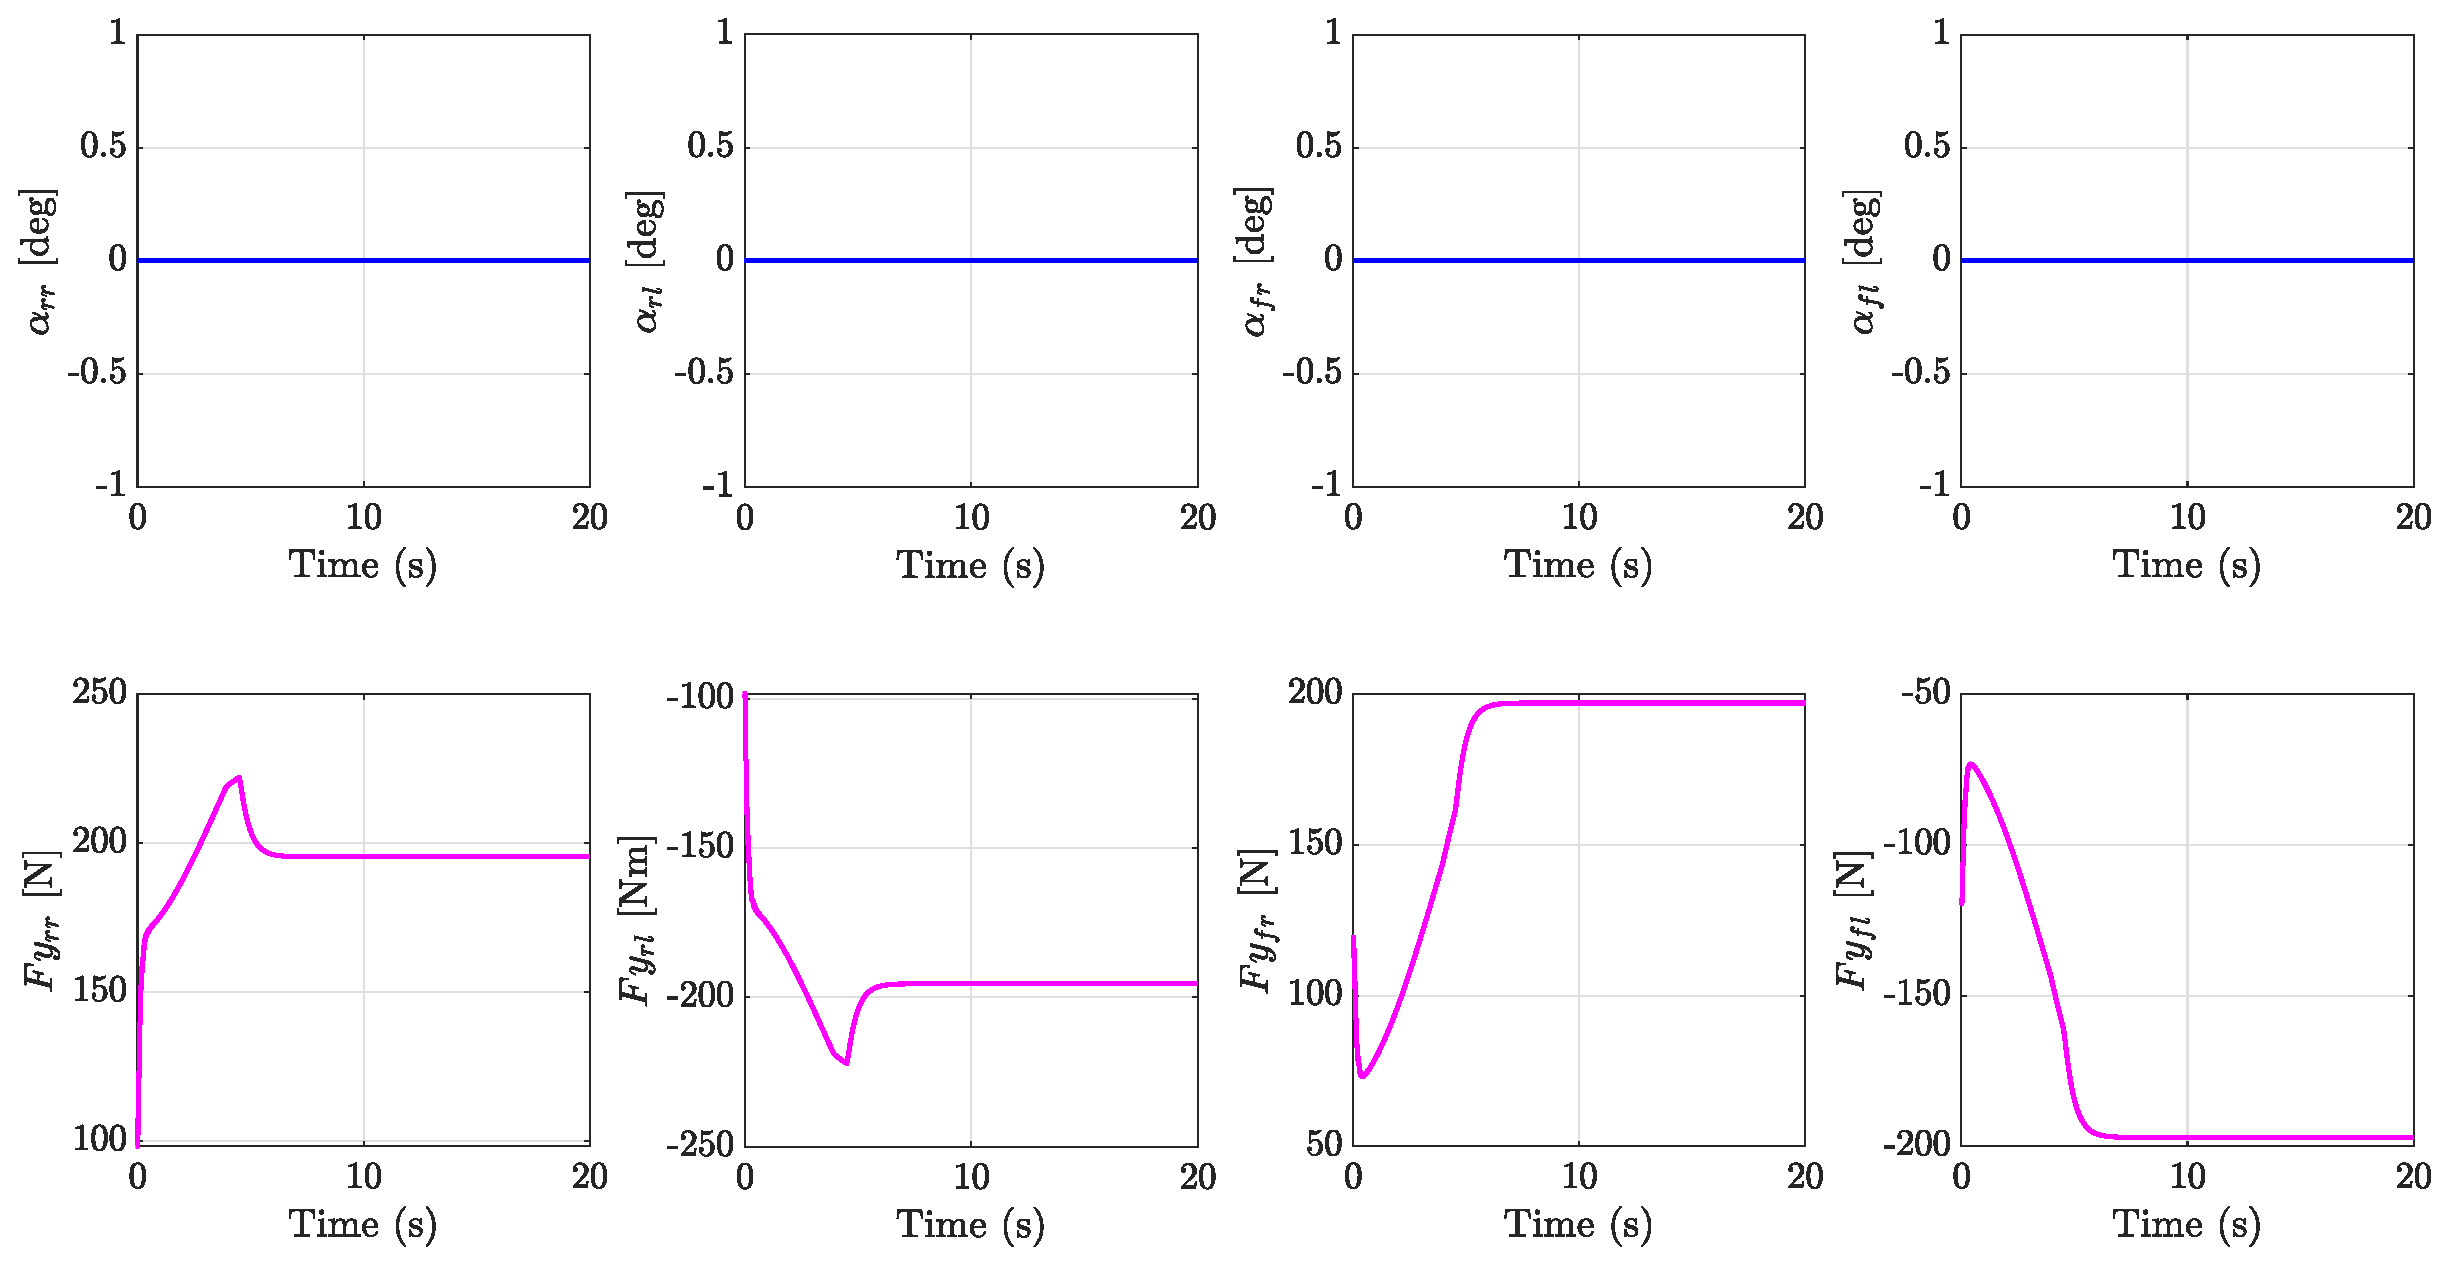
\includegraphics[width=0.85\linewidth]{ex4/q1/ex-41d.eps}
        \centering
        \caption{side slip angle $\alpha$ and lateral forces $\fy$ [maneuver \#1]}
        \label{41d}
        \end{figure}

As previously mentioned, the vehicle has no steering input, which is why the side slip angle $\alpha$ for all tires are zero [Figure \ref{41d}]. Furthermore, the magnitude of the lateral forces on the right tires are equal [and similarly the left tires]. The right tires' lateral forces are opposite in direction compared to the left tires and equal in magnitude, thus making them cancel out keeping the vehicle moving straight. $\fy$\ is smaller than $\fx$\ for all the tires. The self aligning torque $\mz$ profiles previously shown in Figure \ref{41h} resemble the lateral forces profiles for each tire as they are trying to counter their effect on the steering.

During acceleration, the lateral forces $\fy$ across all tires increase because the vertical forces $\fz$ increased. The lateral forces relies on the vertical forces in the pacejka calculations, which is why both the $\fy$ and $\fz$ profiles match for front and rear tires.

% \vspace{-1em}
\newpage
\begin{enumerate}[resume]
  \item initial conditions: $\uz$ = 100 km/h \\
simulation timing: $\ts$\ = 0.001 s, $\tf$\ = 1.5 s \\
requested pedal: req\_pedal = -1 \\
requested steering wheel angle: req\_steer = 0 deg.
  \end{enumerate}

        \begin{figure}[ht]
        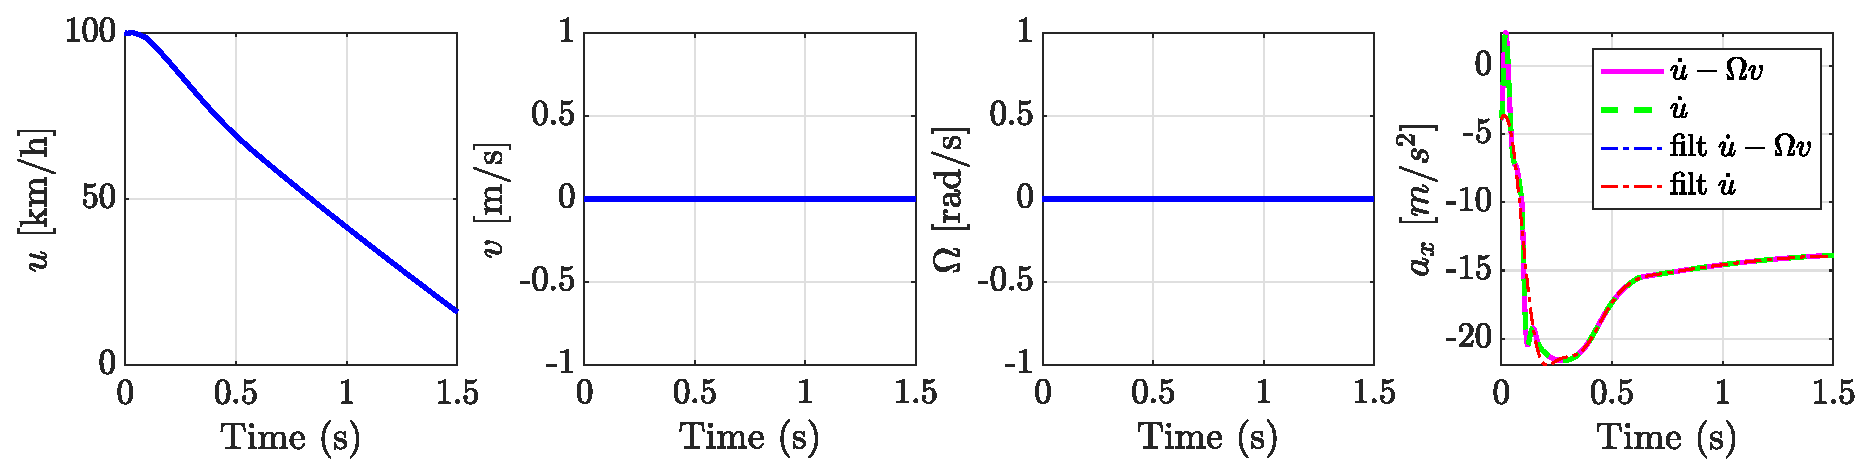
\includegraphics[width=0.99\linewidth]{ex4/q2/ex-42b.eps}
        \centering
        \caption{vehicle motion graphs [maneuver \#2]}
        \label{42b}
        \end{figure}

Figure \ref{42b} shows the motion graphs of the second maneuver. The vehicle starts from 100 km/h, with no steering input and applying full brakes. The velocity dropped to 16 km/h within the specified 1.5 seconds. The deceleration shows a decrease after 0.27 seconds as the rear tires start slipping and going into a full wheel lock as shown in Figure \ref{42f}.

        \begin{figure}[ht]
        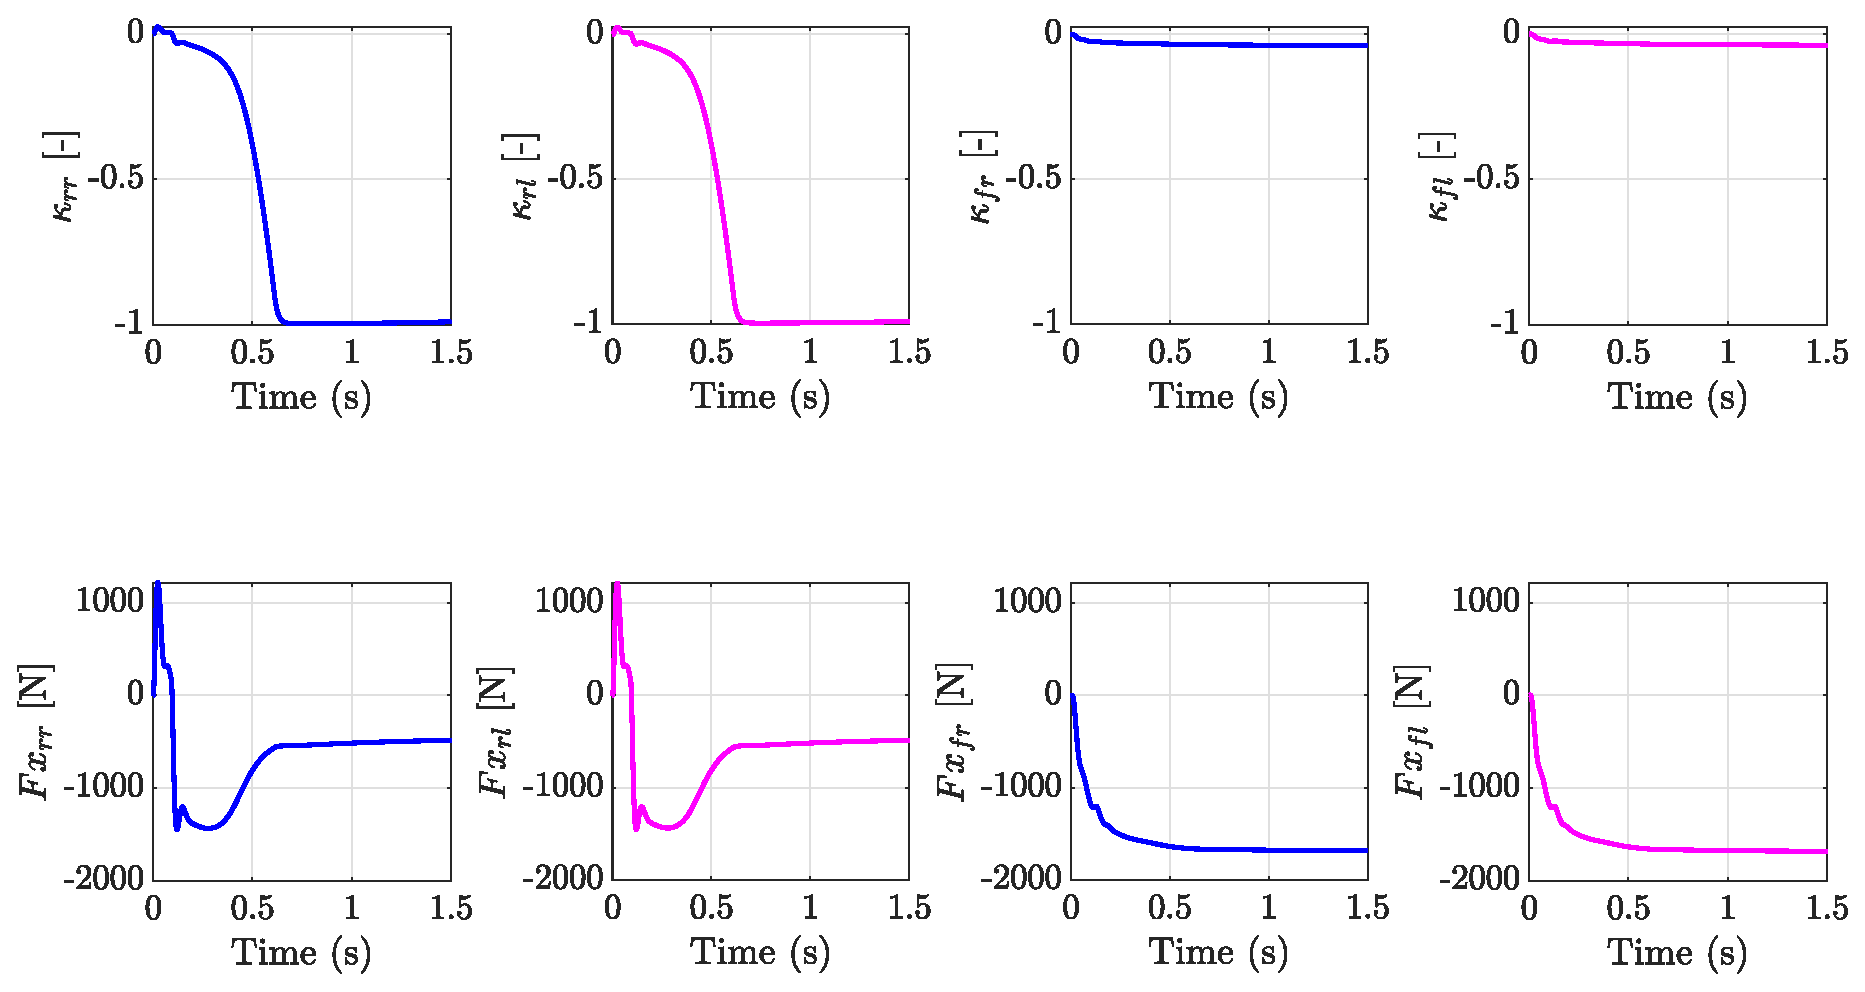
\includegraphics[width=0.85\linewidth]{ex4/q2/ex-42f.eps}
        \centering
        \caption{longitudinal slip $\kappa$ and longitudinal forces $\fx$ [maneuver \#2]}
        \label{42f}
        \end{figure}
        
This maneuver also doesn't have steering input, which is why the graphs in Figure \ref{42f} show no difference between both right and left tires. The longitudinal forces $\fx$ for all tires increase in the opposite direction because the vehicle is decelerating. The longitudinal slip $\kappa$ for the rear tires go to -1, which means both tires went into wheel lock. $\fx$ decreases once wheel lock starts to occur causing lower efficiency in braking and the deceleration rate decreases.

        \begin{figure}[ht]
        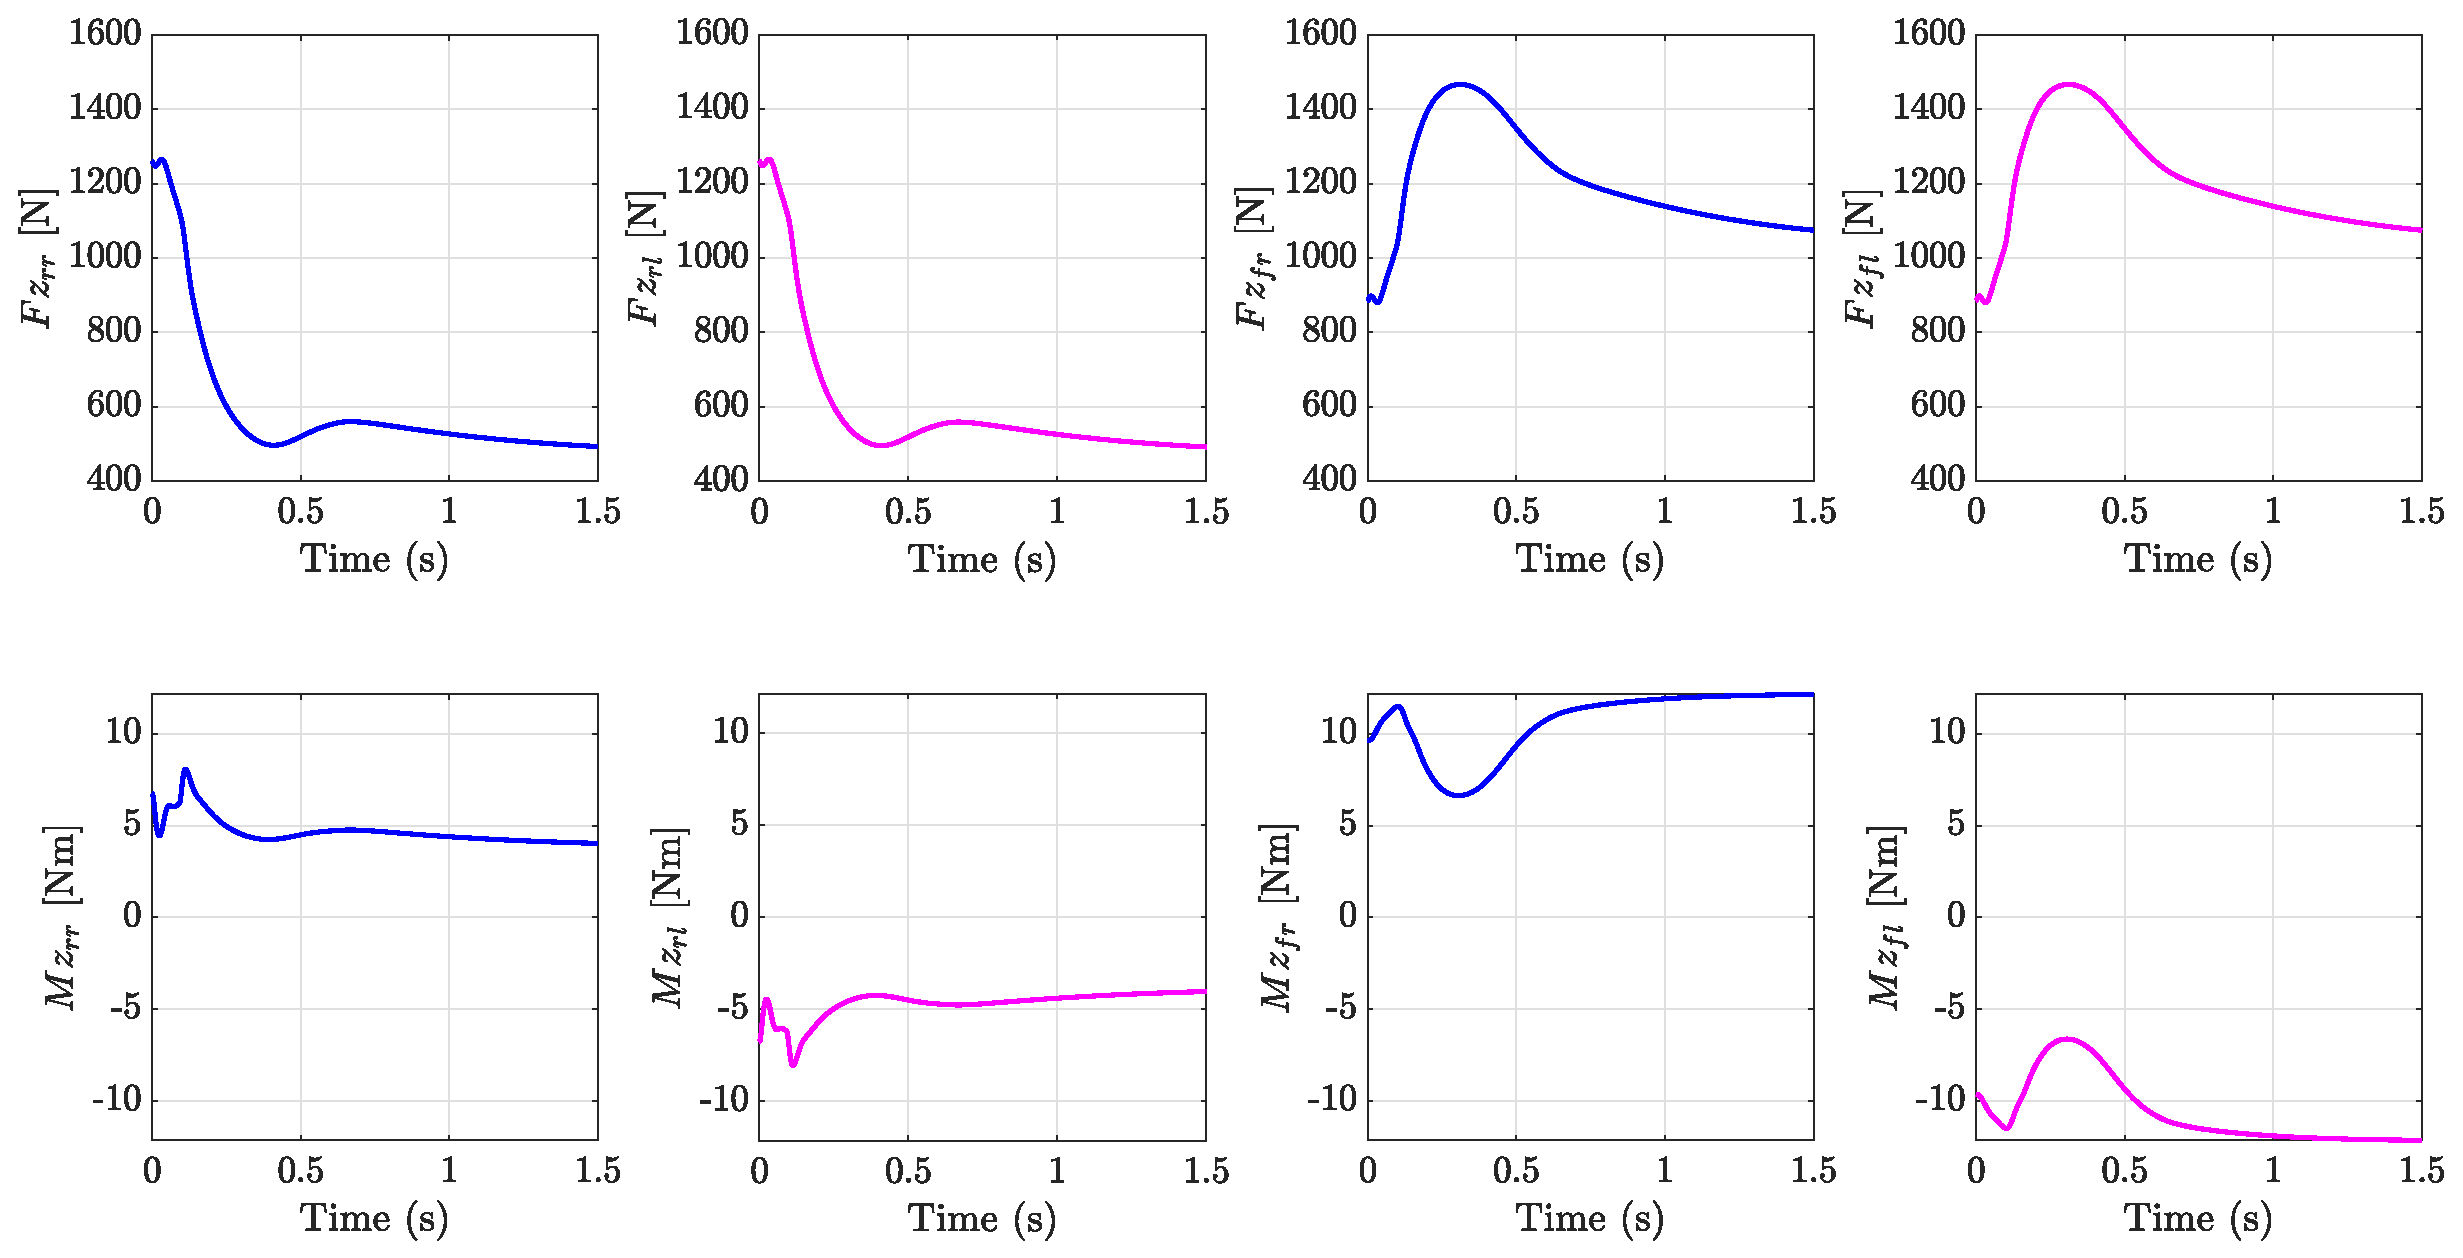
\includegraphics[width=0.85\linewidth]{ex4/q2/ex-42h.eps}
        \centering
        \caption{Vertical forces $\fz$\ and self aligning torque $M_{z}$ [maneuver \#2]}
        \label{42h}
        \end{figure}

Figure \ref{42h} shows the vertical force $\fz$ has decreased in the rear tires while increasing in the front. This is attributed to the longitudinal load transfer to the front because of the braking. The $\fz$ forces on all tires showed a peak around 0.27 seconds due to the rear wheels locking.

No steering input means no side slip angle $\alpha$ for all tires [Figure \ref{42d}]. And similar to maneuver \#1, the right tires' lateral forces are opposite in direction compared to the left tires and equal in magnitude. The self aligning torque $\mz$ profiles in Figure \ref{42h} for each tire are trying to counter the $\fy$'s effect on the steering. $\fy$ showed the same trend as $\fz$, increasing in the front while decreasing in the rear tires.

        \begin{figure}[ht]
        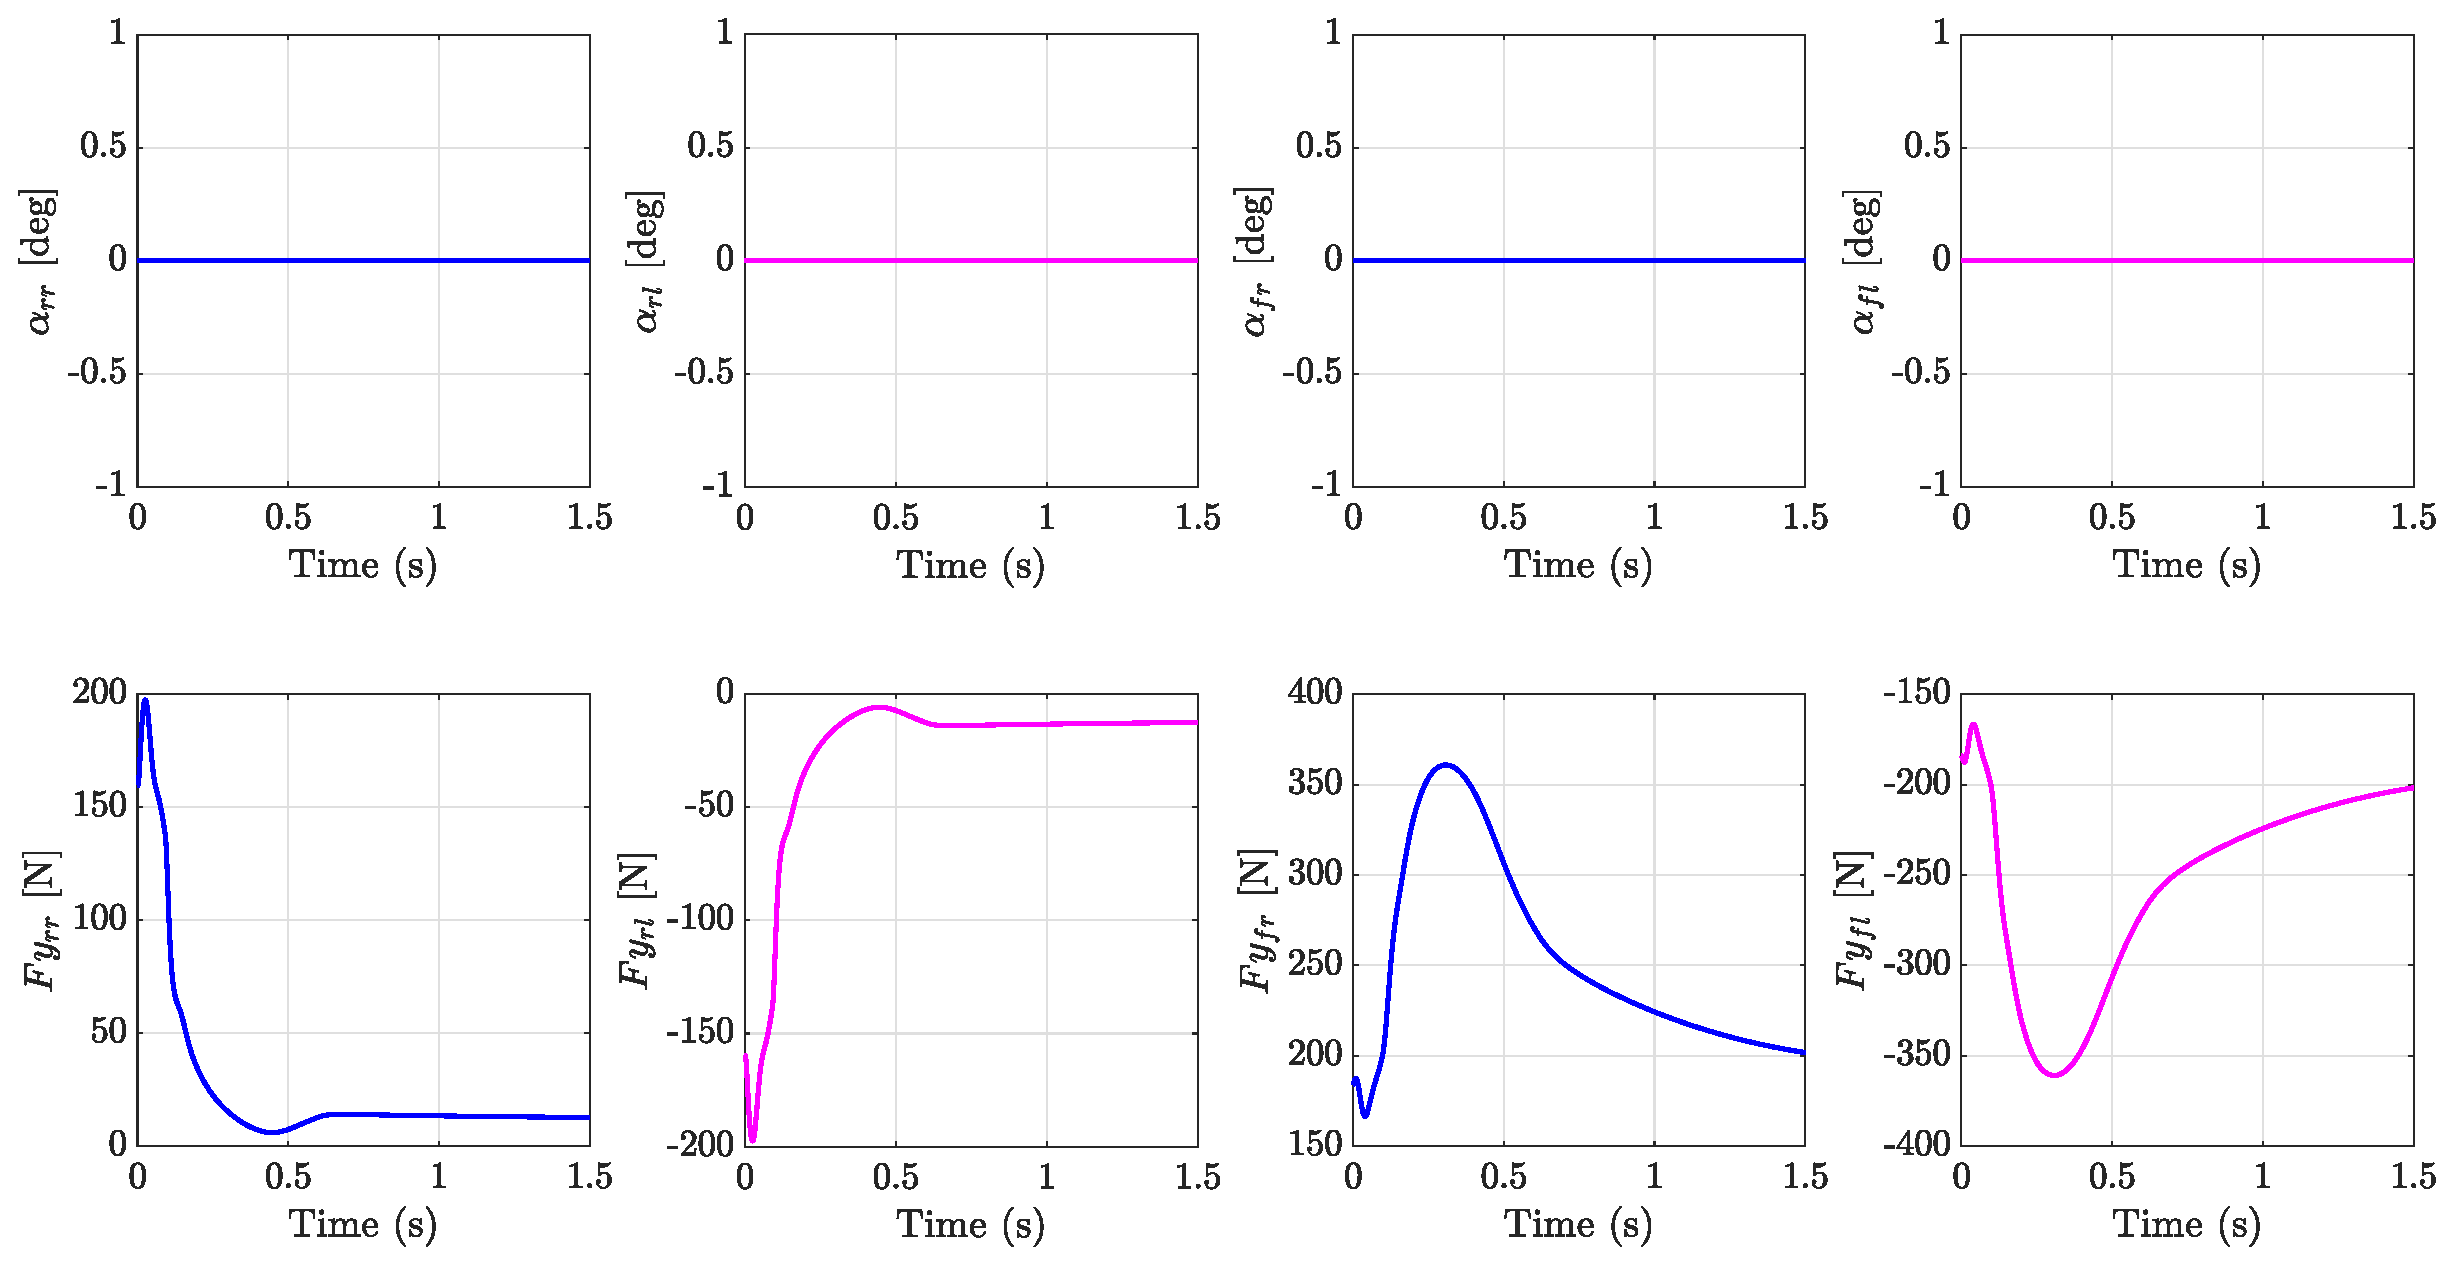
\includegraphics[width=0.85\linewidth]{ex4/q2/ex-42d.eps}
        \centering
        \caption{side slip angle $\alpha$ and lateral forces $\fy$ [maneuver \#2]}
        \label{42d}
        \end{figure}
\newpage
\begin{enumerate}[resume]
  \item initial conditions: $\uz$ = 50 km/h \\
simulation timing: $\ts$\ = 0.001 s, $\tf$\ = 1.5 s \\
requested pedal: req\_pedal = 0.5 \\
requested steering wheel angle: req\_steer = 20 deg.
  \end{enumerate}


        \begin{figure}[ht]
        
\includegraphics[width=0.99\linewidth]{ex4/q3/ex-43b.eps}
        \centering
        \caption{vehicle motion graphs [maneuver \#3]}
        \label{43b}
        \end{figure}

Figure \ref{43b} shows the motion graphs of the third maneuver. The longitudinal speed $u$ keeps increasing until it reaches full saturation for half throttle. The lateral speed $v$ shows the same profile as $u$. $v$ is negative indicating the vehicle is turning left. The yaw rate $\Omega$ follows the same pattern, increasing during acceleration, and constant once acceleration is zero.

        \begin{figure}[ht]
        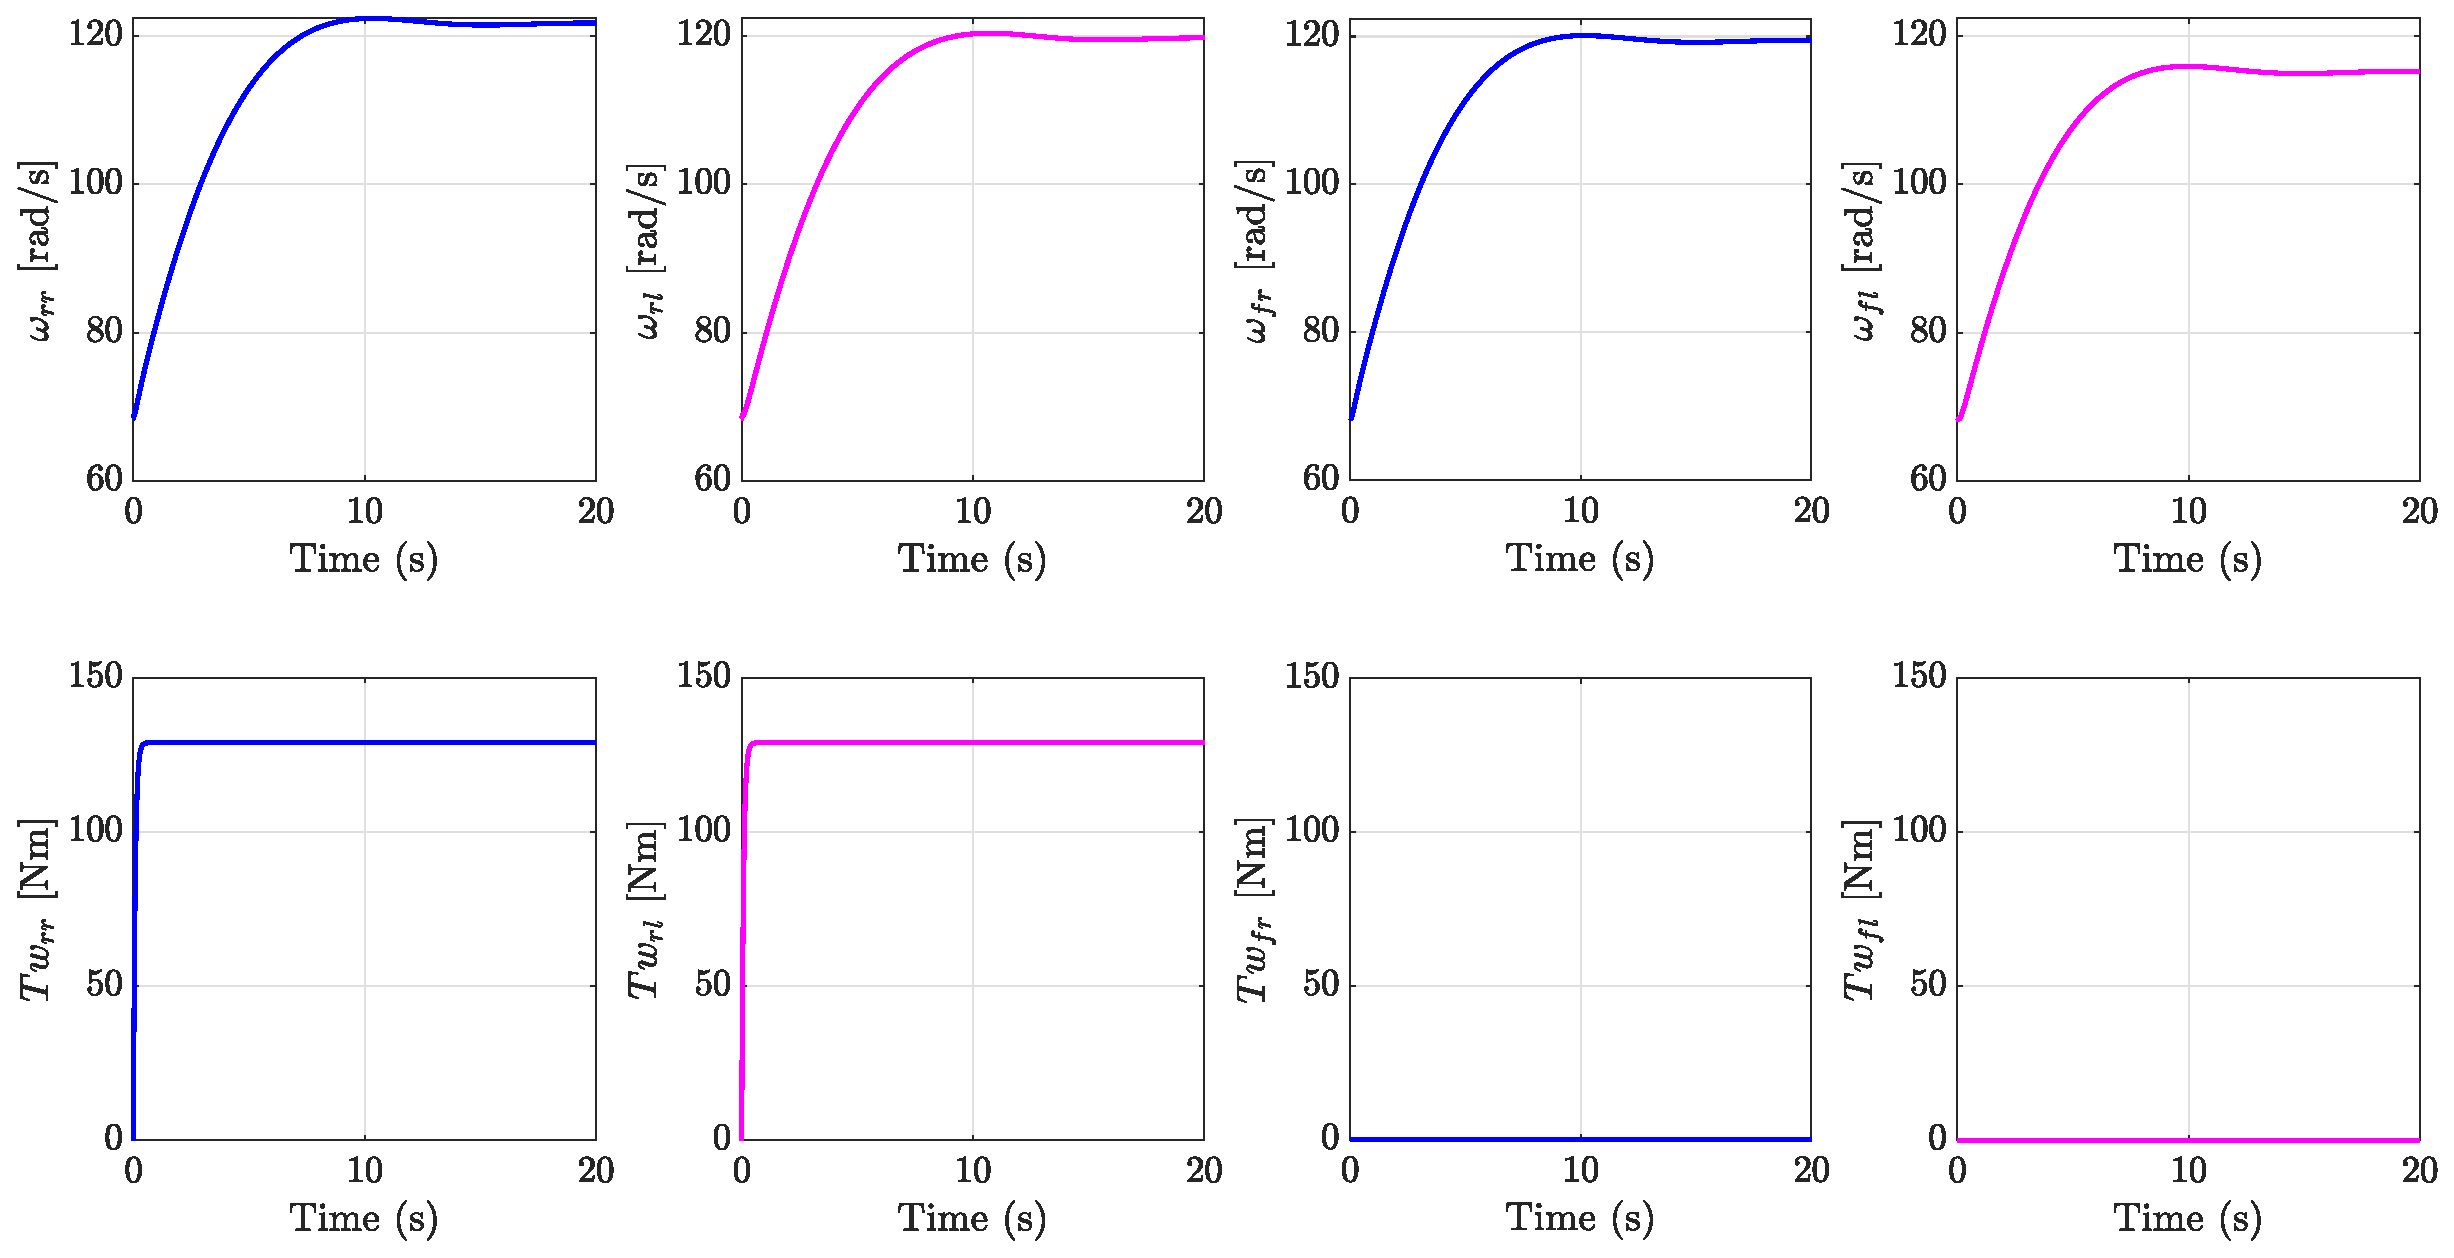
\includegraphics[width=0.88\linewidth]{ex4/q3/ex-43g.eps}
        \centering
        \caption{Wheel rates $\omega$ and Torques $Tw$ [maneuver \#3]}
        \label{43g}
        \end{figure}

The angular velocity $\omega$ are different for different for each wheel as the outer [right] tires would need to rotate faster than the inner [left] tires [Figure \ref{43g}]. The torque experienced by the rear tires are equal to each other, while the front ones are zero.

The longitudinal slip $\kappa$ relies on $\omega$ for each wheel and can be calculated using Equation \ref{eq:4.3}:

\begin{equation}\label{eq:4.3} % add * after equation for unnumbered equations
    \kappa_{ij} = \frac{\omega_{ij} R_{ij} - \upsilon_{cxij} }{\upsilon_{cxij}} \quad i \in \{f,r\} \quad j \in \{r,l\}
\end{equation}

Figure \ref{43f} shows $\kappa$ and $\fx$. As there was no torque on the front tires, $\kappa$ and $\fx$ on the front tires were small. $\kappa$ for the rear tires are different because they are rotating at different speeds. However, both rear tires still experienced the same $\fx$.

        \begin{figure}[ht]
        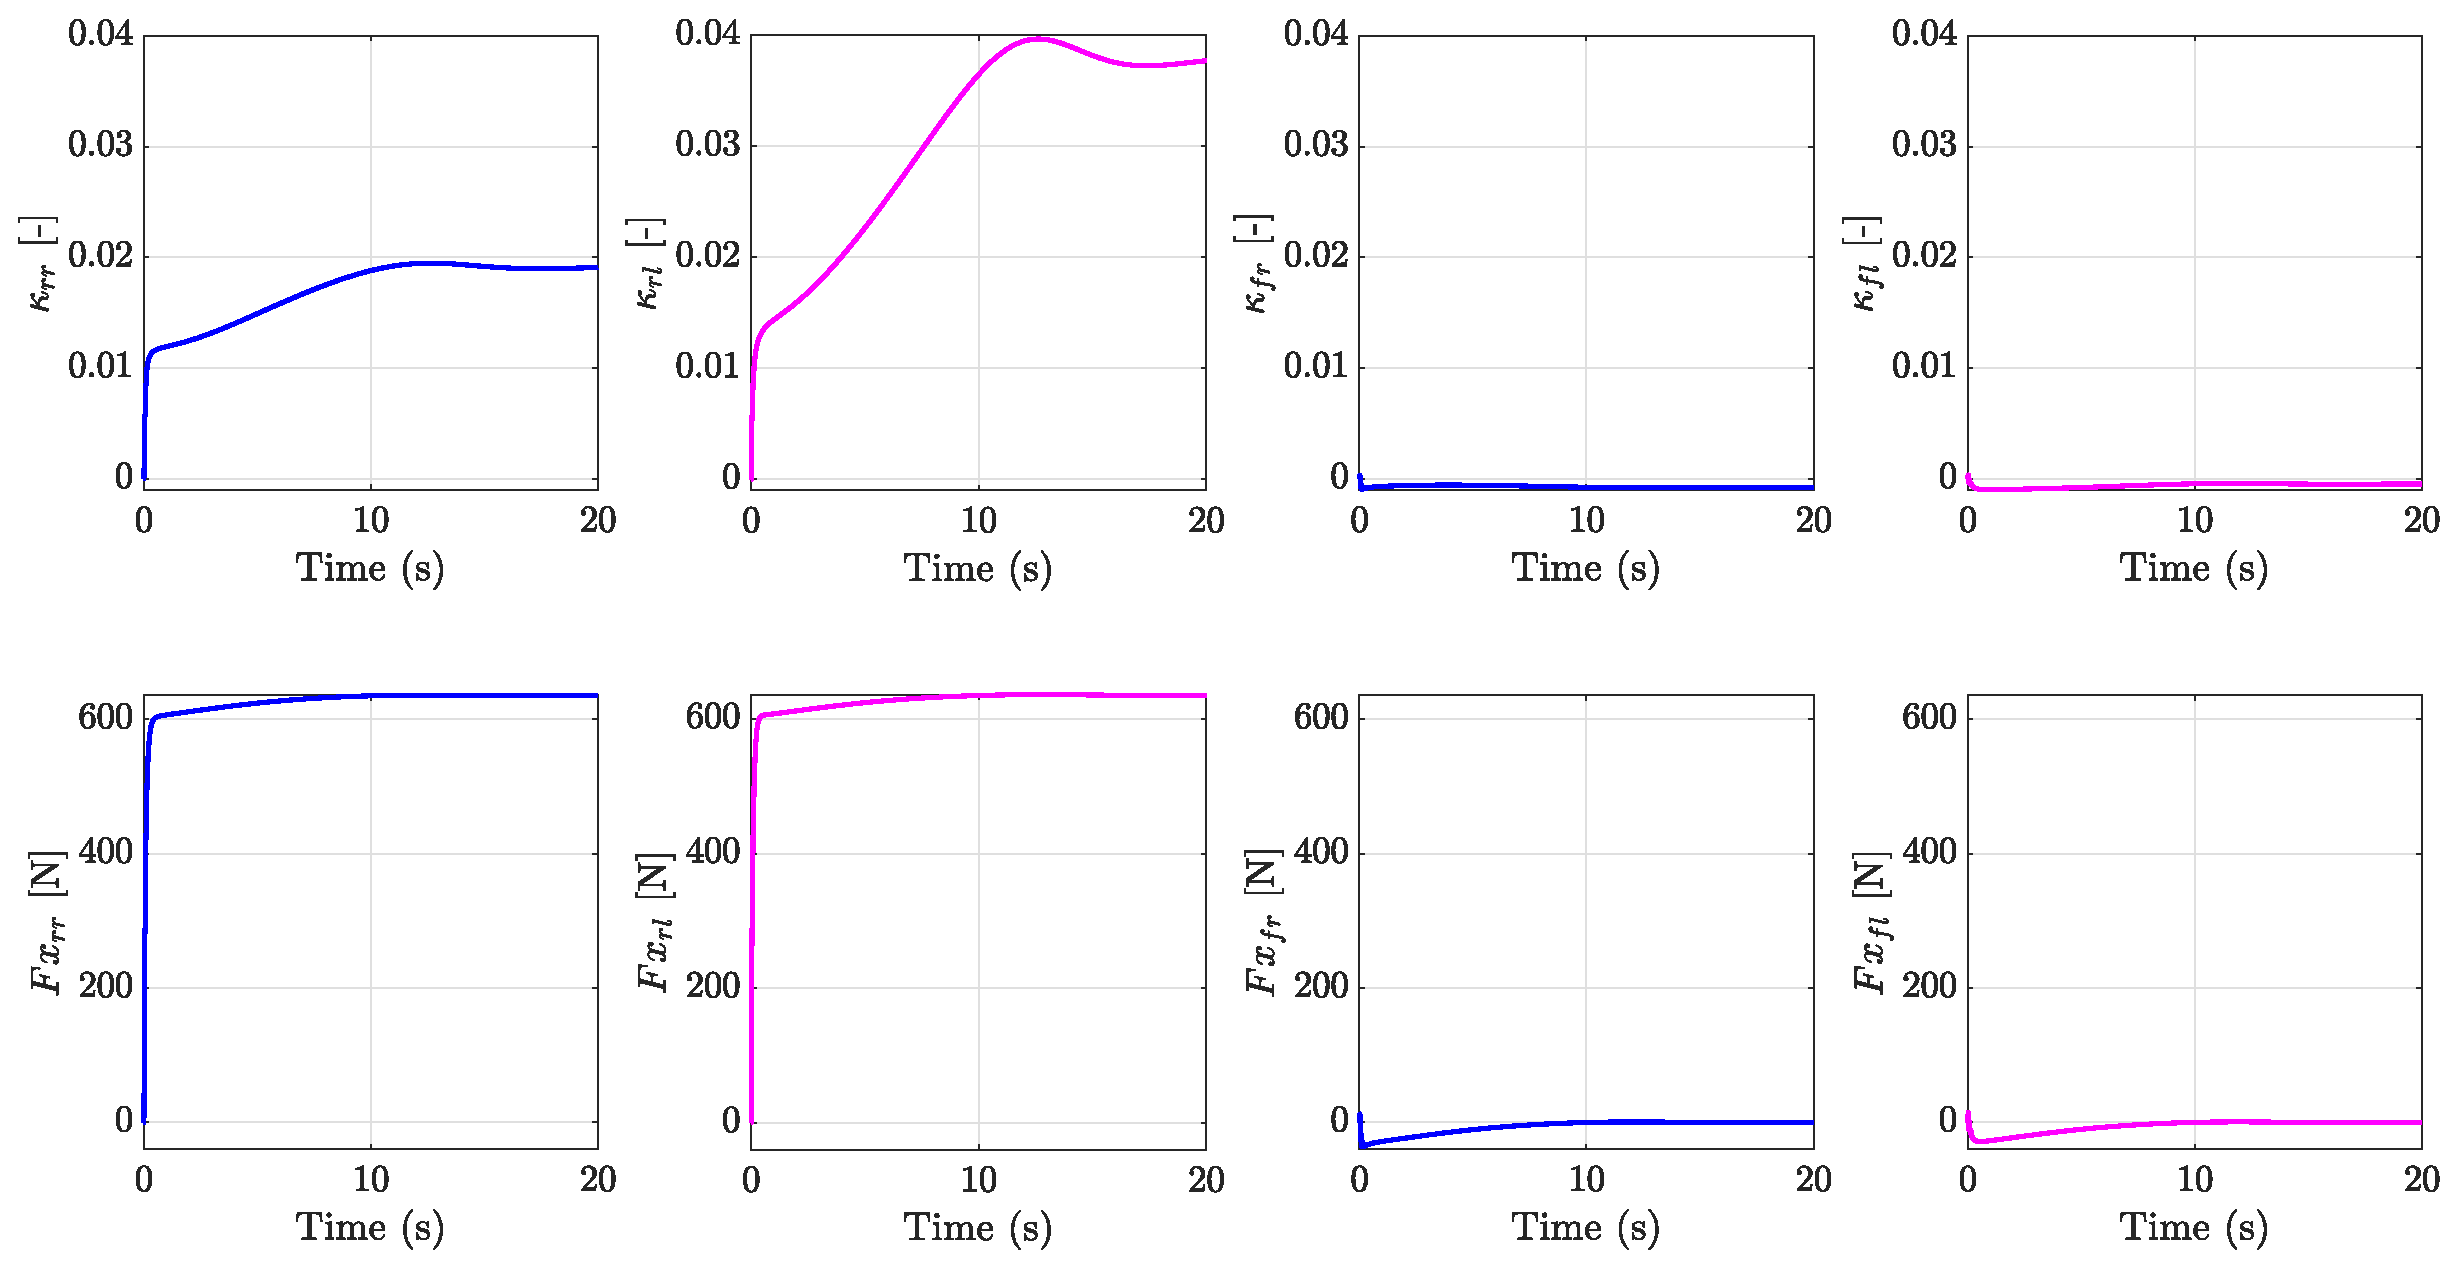
\includegraphics[width=0.88\linewidth]{ex4/q3/ex-43f.eps}
        \centering
        \caption{longitudinal slip $\kappa$ and longitudinal forces $\fx$ [maneuver \#3]}
        \label{43f}
        \end{figure}
        

        \begin{figure}[ht]
        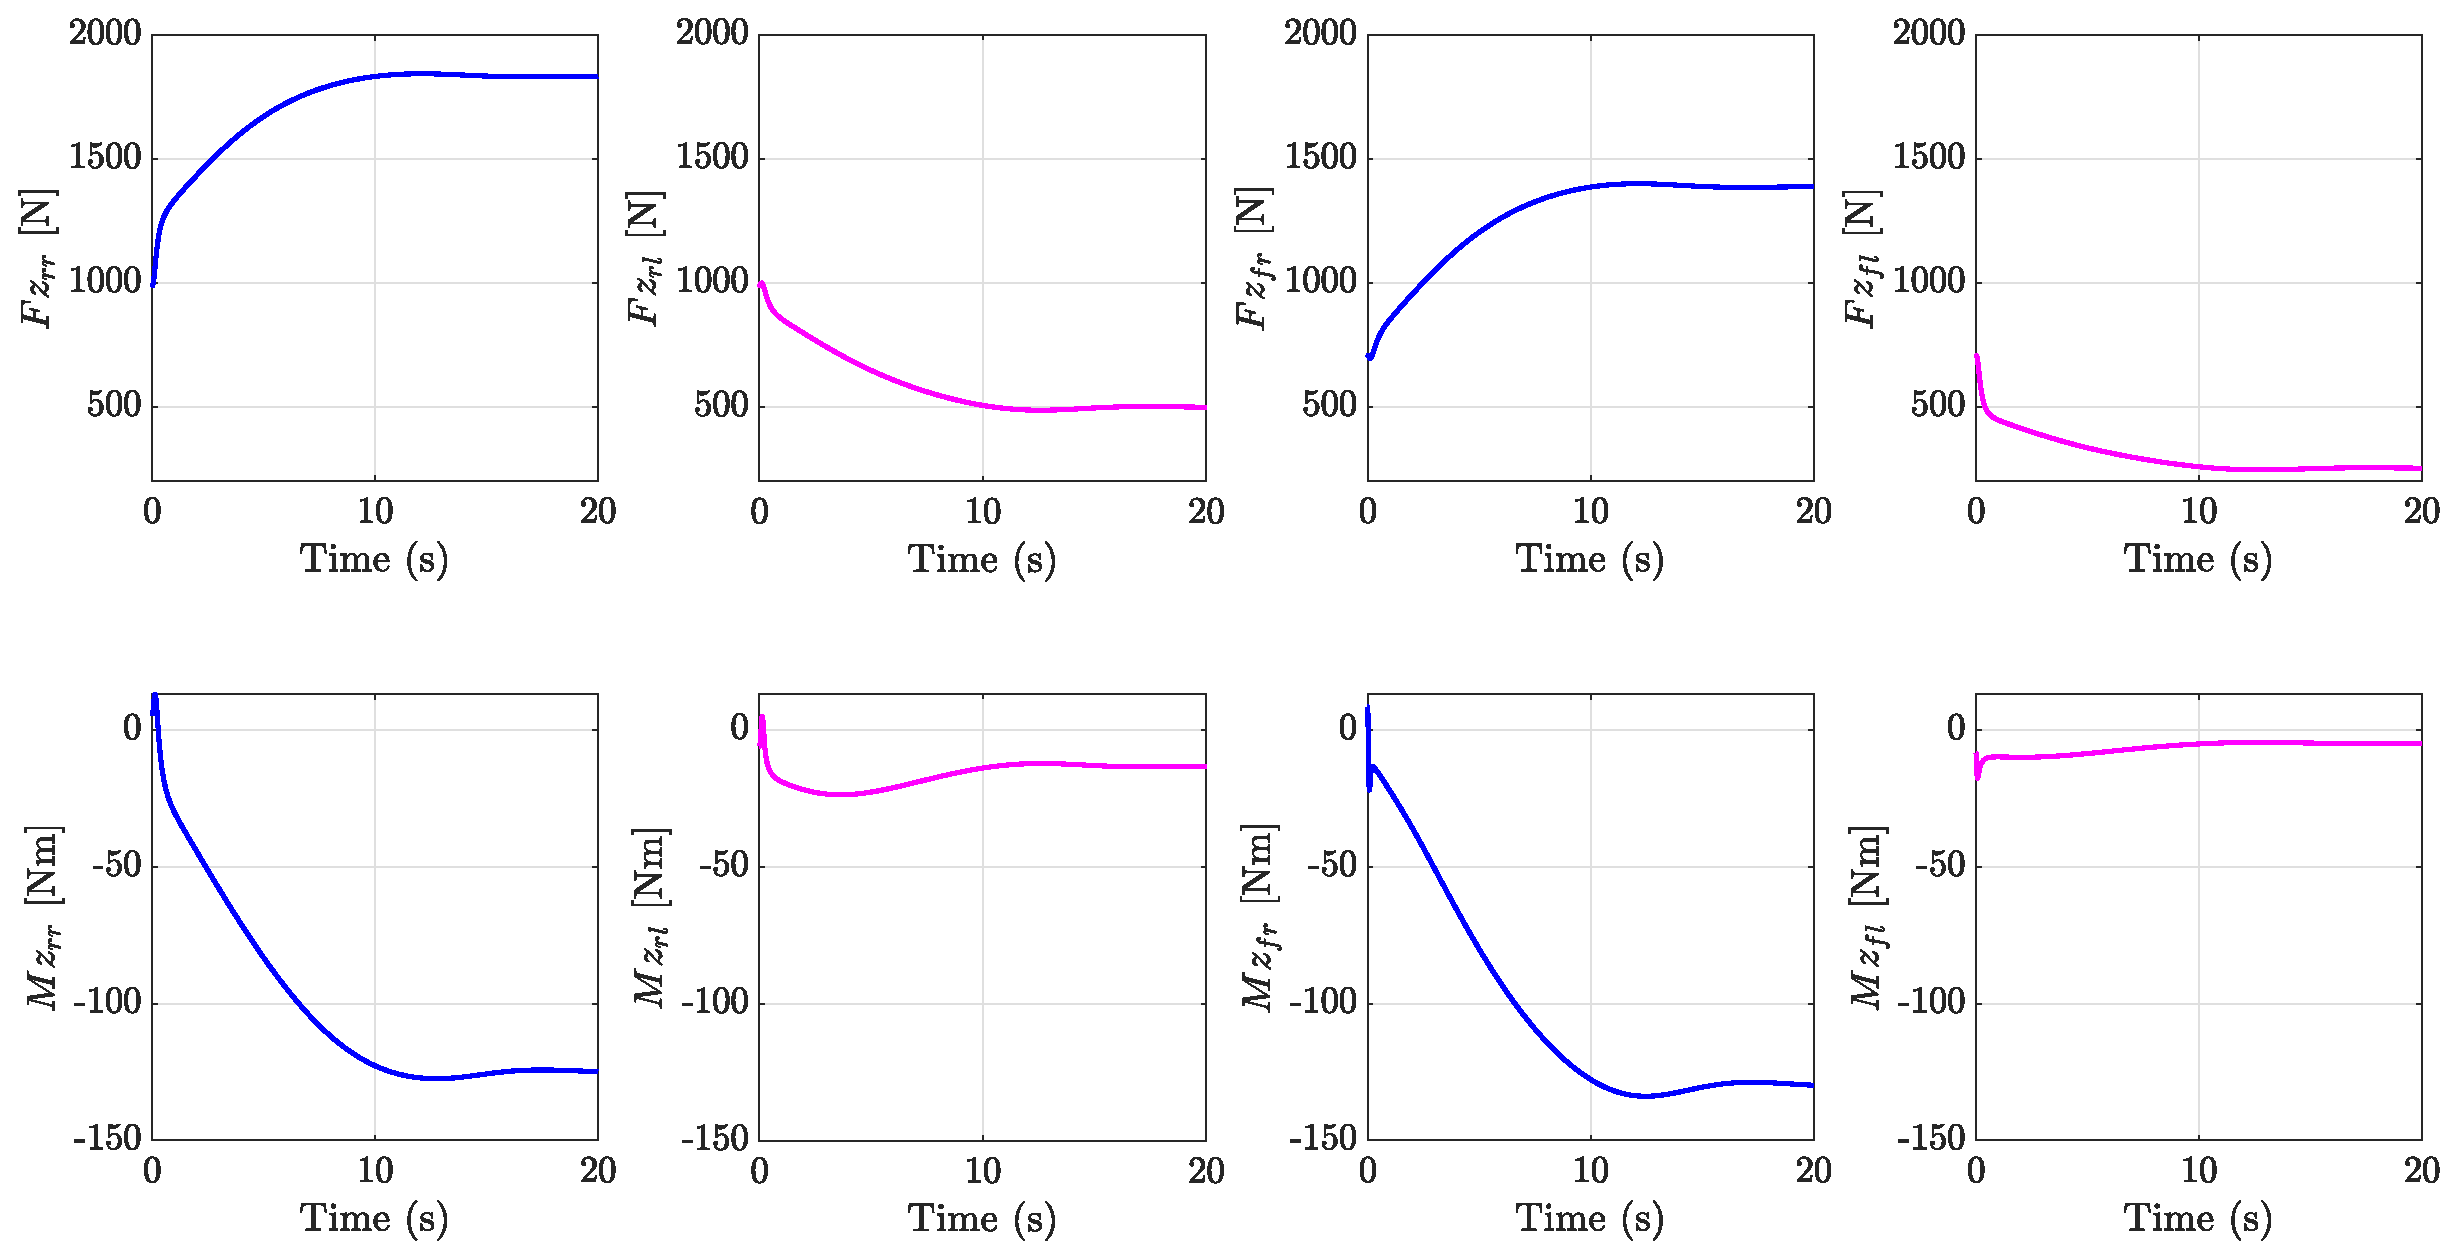
\includegraphics[width=0.88\linewidth]{ex4/q3/ex-43h.eps}
        \centering
        \caption{Vertical forces $\fz$\ and self aligning torque $M_{z}$ [maneuver \#3]}
        \label{43h}
        \end{figure}

Figure \ref{43h} shows the vertical forces $\fz$ for the right [outer] tires increasing then becoming constant when acceleration becomes zero. The left [inner] tires experienced the opposite because of the lateral load transfer to the right side of the vehicle due to the left turn.

The lateral side slip $\alpha$ for all tires are calculated using Equation \ref{eq:4.2}:

\begin{equation}\label{eq:4.2}
    \alpha_{ij} = - \arctan(\frac{vc_{yij}}{vc_{xij}}) \quad i \in \{f,r\} \quad j \in \{r,l\}
\end{equation}

$\alpha$ appears to be consistent across the four tires as shown in Figure \ref{43d}. However, the rear tires are slightly higher due to the torque applied by the motors.

The right side tires have higher lateral forces $\fy$ compared to the right. This is because $\fy$ relies on $\fz$, as the the lateral load transferred to the right side during the left turn maneuver. Both $\alpha$ and $\fy$ become constant once the acceleration is equal to zero. The self aligning torque $\mz$ profiles in Figure \ref{43h} for each tire are trying to counter the $\fy$'s effect on the steering.

        \begin{figure}[ht]
        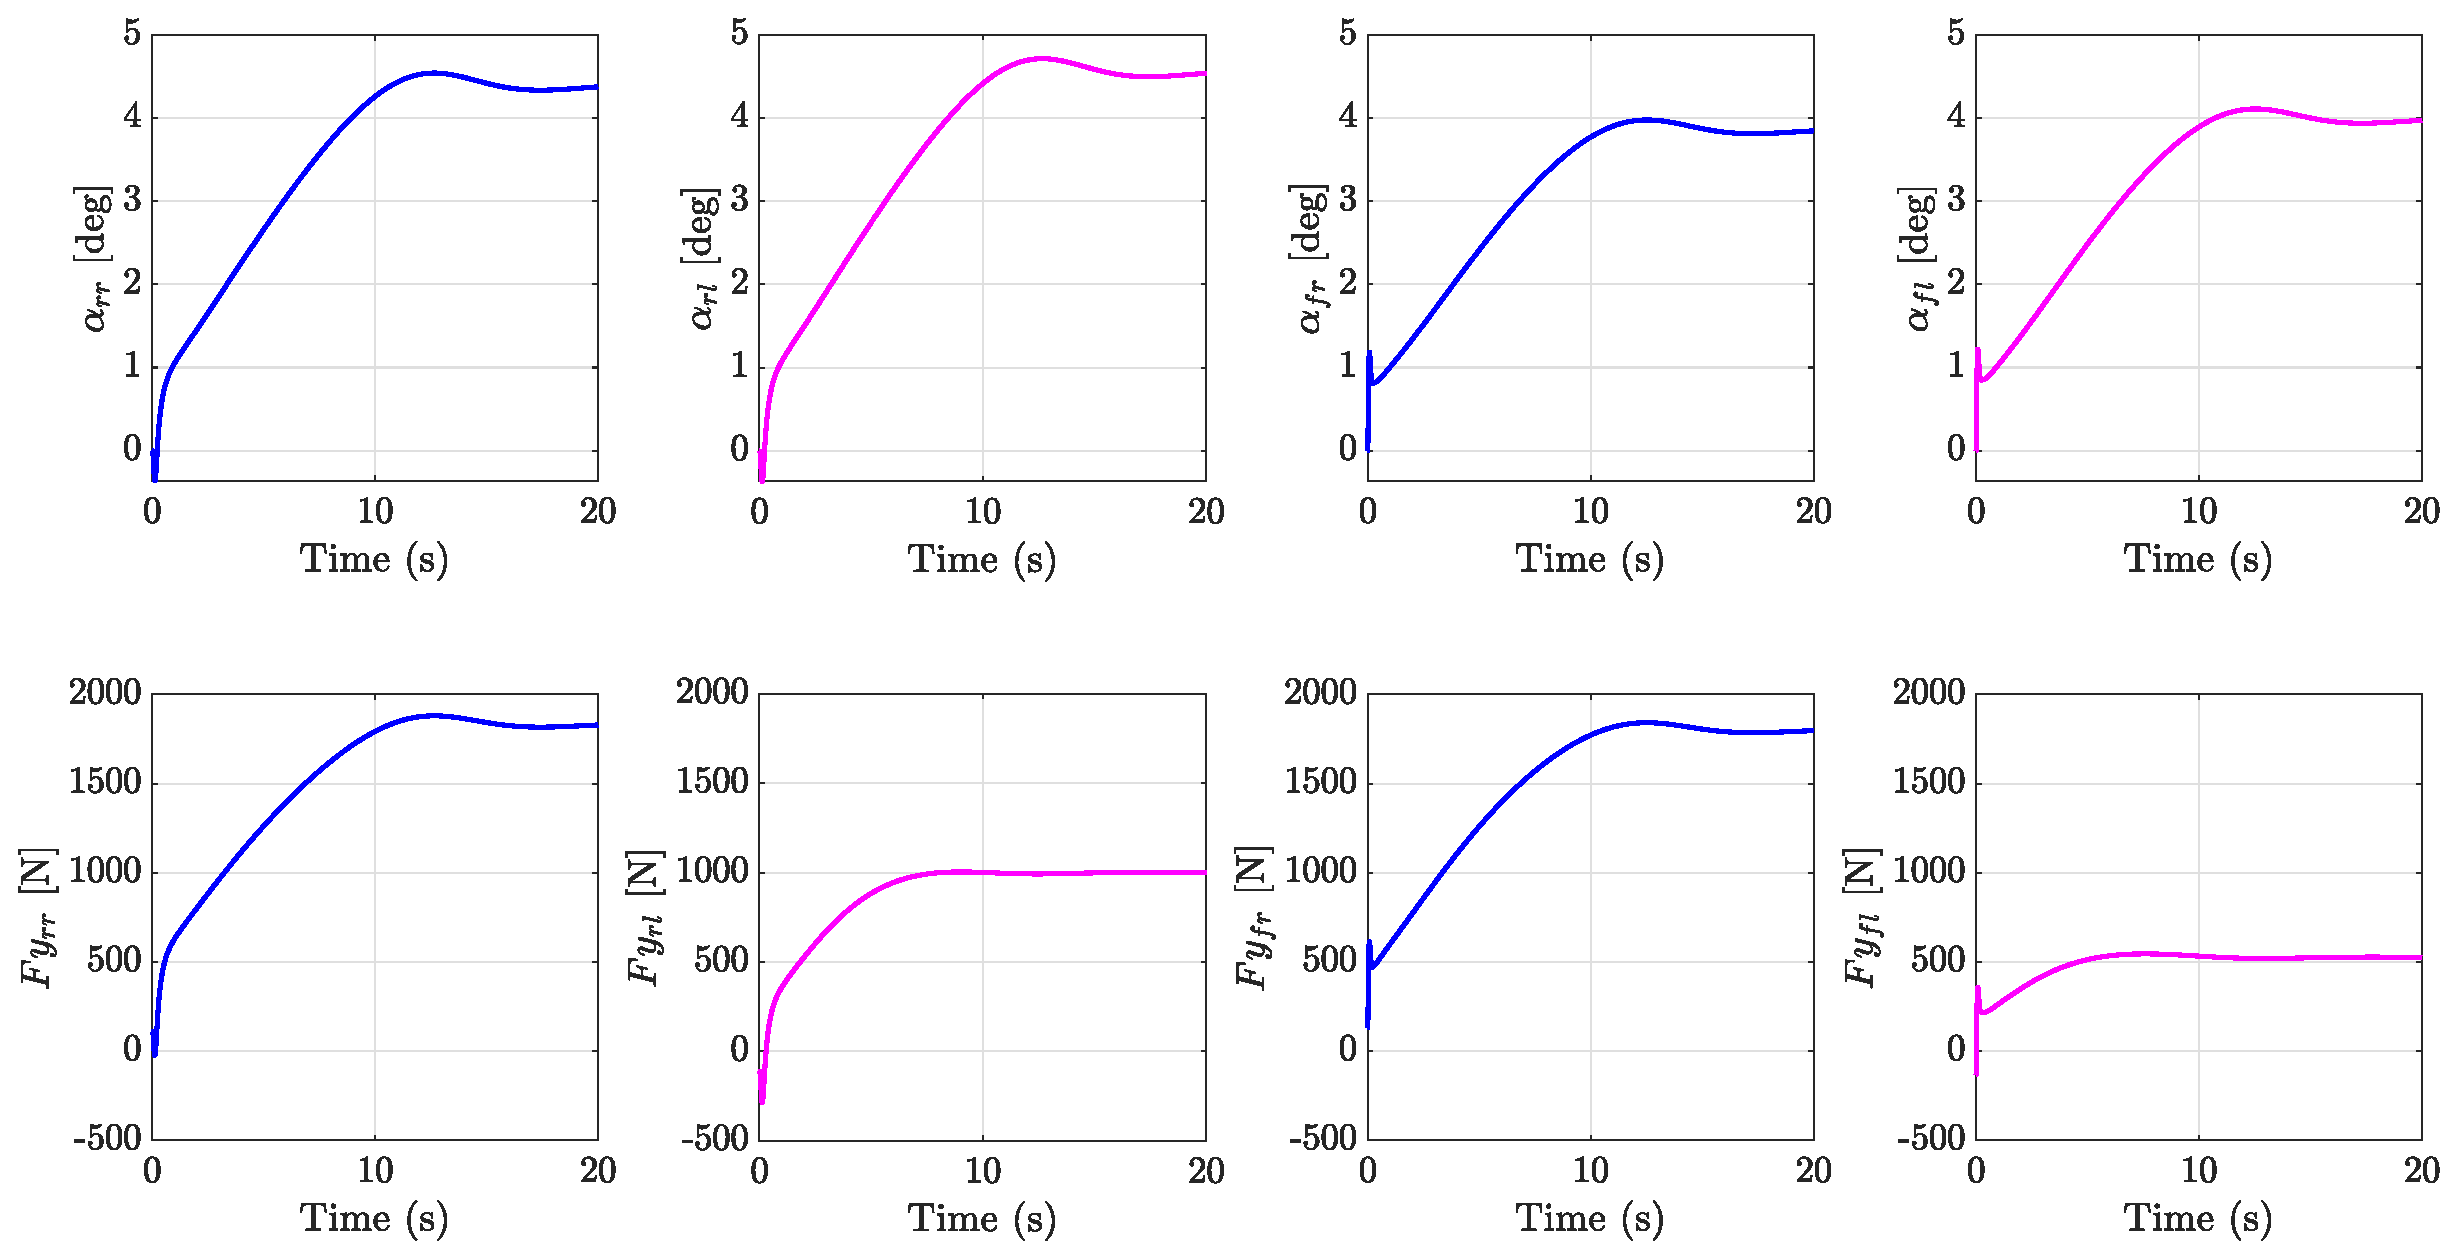
\includegraphics[width=0.88\linewidth]{ex4/q3/ex-43d.eps}
        \centering
        \caption{side slip angle $\alpha$ and lateral forces $\fy$ [maneuver \#3]}
        \label{43d}
        \end{figure}
